% !TEX root = ./../main.tex
\chapter{Introduction to Molecular Dynamics}
For macroscopic bodies, the motion of a system in time and space is governed by the classical equations of
motion, say Newton’s laws, while reducing time and space scales, quantum mechanics kicks in. Despite the latter
statement, classical laws of motion have proved to be a good approximation also at the molecular level, as long
as atoms are massive enough.

In order to predict the time evolution of a complete system, such as the biomolecular system we will treat in
this thesis, Newton’s equations of motion need to be integrated numerically. The necessity of a numerical
integration arises from the complexity of the interactions involved in realistic systems, often nonlinear
functions of positions and momenta of the particles, which makes it impossible to obtain an analytical solution
for the equations of motion.

In the first part of this Chapter the laws of classical and statistical mechanics will be briefly summarized.
Then we will introduce the computational \acf{MD} method and analyze the main aspects of this technique with some
details about the \textit{empirical} \ac{FF}: the container of system model and parameters under study. This
includes the way to consider and treat the inter--particle interactions at \ac{MD} level. Then, coarse--graining
procedure are introduced, with particular attention to the \martini \ac{FF}, the main \ac{FF} used in this thesis
work. Lastly advanced sampling techniques are explained: the \textit{Umbrella Sampling} and
\textit{Metadynamics}. This introductory Chapter are based on the books of Tuckerman \cite{Tuckerman}, Leach
\cite{Leach}, Frenkel and Smit \cite{Frenkel} and Allen and Tildesley \cite{Allen} to which the reader is
addressed for a more complete discussion.

\section{Review of classical mechanics}
Let us consider a system of $N$ particles with mass $m_i$ and coordinates $\vec r_1,\dots,\vec r_N$. According
to the Newton's second low each particle will experience a total force $\vec F_i$ such that
\begin{equation}
	m_i \ddot{\vec{r}}_i = \vec F_i(\vec r_1,\dots,\vec r_N)
	\label{eq:newtonLaw}
\end{equation}
The total force on each particle is defined as
\begin{equation*}
	\vec F_i(\vec r_1,\dots,\vec r_N) = \vec{f}_i^{\ (e)}(\vec r_i) + \sum_{i\ne j}^N \vec{f}_{ij}^{\ (i)}(\vec r_i - \vec r_j )
\end{equation*}
where $\vec{f}_i^{\ (e)}$ is an external force acting on particle $i$ and $\vec{f}_{ij}^{\ (i)}$, which in general
depends only on distance between particle $i$ and $j$, is the inter--particle force that $i$ exerts on $j$ and
\textit{vice--versa}. Equations~\eqref{eq:newtonLaw} are refereed to as \textit{the equations of motion} of the
system; integrating them, with the sets of the \textit{initial conditions} at start time
$t_0$ $\vec r_1(t_0),\dots,\vec r_N(t_0)$ and $\dot{\vec{r}}_1(t_0),\dots,\dot{\vec{r}}_N(t_0)$, the positions
and the velocities of all the particles in the system at any time are known.

Another way to write the equations of motion is to use particles momenta $\vec p_i = m_i \dot{\vec{r}}_i$ and then
the equations~\eqref{eq:newtonLaw} become
\begin{equation}
	\frac{d\vec p_i}{dt} = \vec F_i(\vec r_1,\dots,\vec r_N)
	\label{eq:newtonLawMom}
\end{equation}
The full set of $6N$ functions $(\vec r_1(t),\dots,\vec r_N(t),\vec p_1(t),\dots,\vec p_N)$ gives us a full
description of the dynamics of the $N$--particle system. The set of functions above can be arranged in an ordered
$6N$--dimensional vector
\begin{equation}
	\vec x(t) = (\vec r_1(t),\dots,\vec r_N(t),\vec p_1(t),\dots,\vec p_N)
	\label{eq:phSpaceVector}
\end{equation}
called \textit{phase space vector} or the \textit{microstate} of the system at time $t$. All the possible
microstates of a system generate a $6N$--dimensional space called \textit{phase space} of the system, indicated
with $\Omega$. Thus $\vec x(t)$ describes a particular trajectory in the phase space, i.e. the system evolution
is the motion of a phase space point. For simplicity of notation let us introduce also the ordered vectors
$\vec r = (\vec r_1, \dots, \vec r_N)$, $\dot{\vec r} = (\dot{\vec{r}}_1,\dots,\dot{\vec{r}}_N)$ and
$\vec p = (\vec p_1, \dots, \vec p_N)$ which are the coordinates, velocities and momenta off all particles.

Let us suppose that all the forces acting on the $N$--particle system are conservative; this means that it must
exist a scalar function $U = U(\vec r)$ called \ac{PEF}, such that
\begin{equation}
	\vec F(\vec r) = -\partial_{r_i} U(\vec r)\ \hat e_i = -\vec\nabla_{\vec r} U(\vec r)
	\label{eq:pefForces}
\end{equation}
where $\vec F = (\vec F_1,\dots, \vec F_N)$. Thus we have only to know the \ac{PEF} of the system at any time and
the initial conditions to solve Newton's laws.

The kinetic energy of the system is defined as
\begin{equation}
	K(\dot{\vec r}) = \sum_{i=0}^{N}\frac{1}{2}m_i \dot{\vec r}_i\cdot \dot{\vec r}_i
	\label{eq:kinetic}
\end{equation}

If the system is conservative we can define a scalar function, called \textit{Lagrangian} of the system
\graffito{Lagrangian formalism}
\begin{equation}
	\mathcal{L}(\vec r,\dot{\vec r}) = K(\dot{\vec r}) - U(\vec r)
	\label{eq:lagrangian}
\end{equation}
such that
\begin{equation}
	\frac{d}{dt}\left ( \frac{\partial \mathcal{L}}{\partial \dot r_{i}}\right ) - \frac{\partial\mathcal{L}}{\partial r_{i}} = 0
	\label{eq:EulerLagrange}
\end{equation}
These set of $3N$ equations are called \textit{Euler--Lagrange equations of motion}. It is easy to show that
substituting the definition of $\mathcal{L}$ \eqref{eq:lagrangian} we obtain the Newton's second law. The
Euler--Lagrange equations are a sort of generator of the equations of motion.

Using the definition of $\mathcal{L}$ \eqref{eq:lagrangian} we have
\begin{equation}
	p_i = \frac{\partial\mathcal{L}}{\partial \dot r_i} = m_i\dot r_i
	\label{eq:momentaLagrangian}
\end{equation}
thus we can express particle velocities as a function of particle momenta. Equations~\eqref{eq:kinetic}
and~\eqref{eq:momentaLagrangian} let us to express the kinetic energy in the form
\begin{equation}
	K(\vec p) = \sum_{i=0}^N \frac{1}{2m_i}\vec p_i \cdot \vec p_i
	\label{eq:kineticP}
\end{equation}

To describe the system we can define another scalar function, called \textit{Hamiltonian} of the system
\graffito{Hamiltonian formalism}
\begin{equation*}
	\mathcal{H}(\vec r, \vec p) = \sum_{i=0}^N \vec p_i \cdot \dot{\vec r}_i(\vec p_i) - \mathcal{L}(\vec r, \dot{\vec r}(\vec p))
\end{equation*}
Substituting~\eqref{eq:lagrangian} and using~\eqref{eq:kineticP}, the Hamiltonian of the system is nothing that
\begin{equation}
	\mathcal{H}(\vec r, \vec p) = K(\vec p) + U(\vec r)
	\label{eq:hamiltonian}
\end{equation}
or \textit{the total energy of the system}. To obtain the equations of motion we have to solve \textit{Hamilton's equations}
\begin{equation}
	\begin{aligned}
		\dot r_i &=& &\frac{\partial\mathcal{H}}{\partial p_{i}} \\
		\dot p_i &=&-&\frac{\partial\mathcal{H}}{\partial r_{i}}
	\end{aligned}
	\label{eq:eqhamilton}
\end{equation}
Describing the system with the Hamiltonian formalism, in some cases, is more useful than Lagrangian one, first of
all because the Hamiltonian of a system is directly related to a well know physical quantity, the total energy.

\section{Review of statistical mechanics}
\label{sec:statmec}
Using the picture of the classical mechanics described above we have a good and sophisticated machinery that
allows us, knowing some information about the system in exam, i.e. initial positions and velocities of all
particles and their interactions, to completely solve the equations of motion in order to get the dynamics of the
system at every time. So classical mechanics encodes all the information about the \textit{microscopic} view of a
system and, in principle, we can extract all the information we want about the \textit{macroscopic} proprieties
of such system. The main task of this process is to obtain the thermodynamics proprieties of a system
(temperature, pressure and so on) from the complete sets of positions and velocities of all particles and thus it
is necessary to have a link between microscopic and macroscopic world.

The solution of that problem comes from \textit{statistical mechanics} developed, principally, by Boltzmann and
Gibbs. Statistical mechanics involves all the rules and methods through which the microscopic and macroscopic
worlds are related to each other. This provides also a rigorous derivation of thermodynamics from the microscopic
proprieties: without that thermodynamics would be only a phenomenological theory. The first step to the solution
of the problem is to recognize that \textit{a macroscopic observable of a system does not strongly depend on the
complete dynamics of each particle in the system, but rather on an average that cancels out all the details of
the microscopic features}. This it is intuitively true. We can think to set up an experiment with a system in a
specific microscopic state that corresponds to a macroscopic state. Certainly we can do the contrary and for sure
we will not find the same microscopic state. Then we can iterate the experiment and we will find that for a
specific macroscopic state of a system there exists a number of microscopic states that yield to the same
properties.

The most important concept that makes this idea practicable is the \textit{statistical ensemble}. Based on the
previous considerations, a general definition of an ensemble is \textit{a collection of systems subject to a set
\graffito{statistical ensemble concept}
of common interactions and sharing the same macroscopic properties}. This concept lays the foundations of
thermodynamic and suggests a procedure to compute many macroscopic observables. In more details a
$N$--particle system in a specific microscopic state is described by its microstate $\vec x$, then \textit{an
ensemble is a set of points in the phase space that are subject to the constraint to be part of the ensemble
itself}. Each system evolves in time with the equations of motion, so the time evolution of an ensemble is
described by the flow of a set of points in the phase space according to the classical mechanics.

Once an ensemble is defined we are able to compute, at every time, the macroscopic observables simply averaging
over all systems in the ensemble. To do this we have to know, at every time, which microstates of the phase space
are part of the ensemble. For this purpose we define the \textit{ensemble distribution function}
$\tilde\rho = \tilde\rho(\vec x,t)$. Let $dx = dr_1\cdots dr_{3N} dp_1 \cdots dp_{3N}$ the infinitesimal phase
space volume, then
\begin{equation*}
	\frac{1}{\mathcal{N}}\tilde\rho(\vec x, t)\ dx = \rho(\vec x, t)\ dx ????
\end{equation*}
where $\mathcal{N}$ is the total number of microstates in the ensemble, $\rho(\vec x, t)dx$ can be interpreted as
the probability to find a system in the ensemble with microstate $\vec x$ at a time $t$ and $\rho(\vec x, t)$ is
the more convenient normalized ensemble distribution function. For definition of probability density must be
\begin{equation*}
	\int_{\Omega} \rho(\vec x, t)\ dx = 1, \qquad \rho(\vec x, t) \ge 0
\end{equation*}

Giving the ensemble distribution function, the ensemble average of an observable $A=A(\vec x)$, at every time, is
defined as
\begin{equation*}
	\ave{A}(t) = \int_\Omega A(\vec x)\rho(\vec x, t)\ dx
\end{equation*}
For an ensemble at thermodynamic equilibrium the macroscopic state is fixed and so, if $A$ is an equilibrium
observable, it must be time--independent. Thus, it can be shown \cite{Tuckerman} that exist a scalar function of
the Hamiltonian $\mathit{f}(\mathcal{H}(\vec x))$ such that the time--independent ensemble average of the
equilibrium observable $A$ can be expressed as
\graffito{ensemble averages}
\begin{equation*}
	\ave{A} = \frac{1}{\mathcal{Z}} \int_\Omega A(\vec x, t) \mathit{f}(\mathcal{H}(\vec x))\ dx
\end{equation*}
where $\mathcal{Z}$, known as \textit{partition function}, is specific for the ensemble in exam and it is defined
as follow
\begin{equation*}
	\mathcal{Z} = \int_\Omega \mathit{f}(\mathcal{H}(\vec x))\ dx
\end{equation*}

In order to compute the partition function we need to specify the thermodynamic observables, called
\textit{control variables}, that characterize the ensemble itself. By definition of an ensemble at thermodynamic
equilibrium those control variables must be constant in time. The main ensembles used in statistical mechanics
and the related control variables are summarized as follow
\begin{itemize}
	\item \textit{microcanonical ensemble}: constant--$NVE$
	\item \textit{canonical ensemble}: constant--$NVT$
	\item \textit{isothermal--isobaric ensemble}: constant--$NpT$
	\item \textit{grand--canonical ensemble}: constant--$\mu pT$
\end{itemize}
The averages computed in different ensembles are equivalent in the so called \textit{thermodynamic limit}: this
is the \textit{equivalence of ensembles}. Thus, it must be possible to change from one ensemble to another
leaving averages unchanged.

We have defined ensemble averages and how to compute them but we need also a link between statistical averages
and the experimental values. When we measure a macroscopic observable $A$ we prepare an experiment with
\textit{only one} system in a specific macroscopic state and we study its evolution in time. $A$ is a function of
time and phase space vector and it fluctuates over time due to particle interactions. The measurement itself
requires long time intervals compared to microscopic time scales, thus when we measure an observable we take an
\textit{average over time}. If, in principle, the time for average is infinity then we have the ``real'' mean
value of the observable
\begin{equation*}
	\overline{A} = \lim_{\tau\to +\infty}\frac{1}{\tau}\int_{t_0}^\tau A(\vec x_t)\ dt
\end{equation*}
In order for a comparison to be made, an identity between ensemble and time averages must be established.
This link is provided by the \textit{ergodic theorem} and the \textit{ergodic hypothesis}. A system is said to be
\graffito{ergodic theorem and ergodic hypothesis}
ergodic if, over a long period of time, all the microstates in the phase space with the same energy are
accessible with the same probability. Then the ergodic theorem says that, if the system is ergodic, the time and
ensemble averages are equal \textit{almost everywhere} in the phase space. So we can write the follow identity
\begin{equation}
	\overline{A} = \lim_{\tau\to +\infty}\frac{1}{\tau}\int_{t_0}^\tau A(\vec x(t))\ dt = \int_\Omega A(\vec x)\rho(\vec x, t)\ dx = \ave{A}(t)
	\label{eq:ergotic}
\end{equation}

For biomolecular applications the most important ensembles are the microcanonical and the isothermal--isobaric.
In the following we will describe them briefly with particular attention to the isothermal--isobaric ensemble,
the most relevant for this thesis work.

\subsection{Microcanonical ensemble}
The microcanonical ensemble is composed of the systems whose number of particles ($N$), volume ($V$) and energy
($E$) are constant. Due to the constant energy it describes a Hamiltonian system for which
\begin{equation*}
	\mathcal{H}(\vec x) = E
\end{equation*}
this let us to define the partition function as follow
\begin{equation}
	\mathcal{Z}_{NVE} = \frac{1}{N!h^{3N}}\int_\Omega \delta(\mathcal{H}(\vec x) - E)\ dx
	\label{eq:micropartition}
\end{equation}
where the normalization factor $N!$ takes into account the particles indistinguishability and $h^{3N}$ is for
compatibility of statistical mechanics with quantum mechanics: it comes from Heisenberg’s uncertainty principle
and it is the smallest phase space volume element. The right thermodynamic potential, i.e. the constant of
motion, to obtain all the macroscopic observables is the entropy $S$ given by
\begin{equation*}
	S = k_B \ln \mathcal{Z}_{NVE}
\end{equation*}
where $k_B = 1.3806505(24) \cdot 10^{-23}$~J/K is the Boltzmann constant. The other thermodynamic quantities can
be obtained by
\begin{equation*}
	\frac{1}{T} = \left ( \frac{\partial S}{\partial E}\right )_{NV} \qquad \frac{p}{T} = \left ( \frac{\partial S}{\partial V}\right )_{NE} \qquad \frac{\mu}{T} = \left ( \frac{\partial S}{\partial N}\right )_{VE}
\end{equation*}

The link between microscopic functions of phase space points and macroscopic observables, like kinetic energy or
pressure, is provided by the \textit{classical virial theorem} which states that
\begin{equation}
	\ave{x_i\frac{\partial\mathcal{H}}{\partial x_k}} = k_B T \delta_{ik}
	\label{eq:virial}
\end{equation}
where $x_i$ is some phase space variable.
% often the virial theorem is written in a slightly different form
% \begin{equation}
% 	\ave{K} = - \frac{1}{2}\sum_{i=1}^{3N} \ave{F_ir_i}
% \end{equation}
% where $\ave{K}$ is the average kinetic energy, not necessary at equilibrium and $F_i$ is the total forces acting on particle $i$. Both are valid even if the system is not at the equilibrium.

\paragraph{\textbf{Kinetic energy}} Since a system in a microcanonical ensemble is defined to be Hamiltonian,
from equations~\eqref{eq:hamiltonian} and~\eqref{eq:kineticP} according to the virial theorem with the choice
$x_i = p_{i}$ we obtain
\begin{equation*}
	\ave{\frac{p^2_{i}}{m_i}} = k_bT
\end{equation*}
then summing both side over all particles and over the three coordinates we obtain the average kinetic energy at
equilibrium
\begin{equation}
	\ave{K} = \ave{ \sum_{i=1}^{N}\sum_{\alpha=1}^{3}\frac{p_{i+\alpha}^2}{2m_i} } = \ave{\sum_{i=1}^{N}\frac{\vec p_i\cdot \vec p_i}{2m_i}} = \frac{3}{2}Nk_B T
	\label{eq:kineticT}
\end{equation}
this is like the well know equipartition theorem in which $3N$ is the number of \ac{DOF}.

\paragraph{\textbf{Pressure}} Choosing $x_i = r_i$ in equation~\eqref{eq:virial} and summing both side over all
particles and substituting equations~\eqref{eq:eqhamilton} and~\eqref{eq:kineticT}, we obtain
\begin{equation*}
	W = \ave{\sum_{i=1}^{3N} r_i\dot p_i} = -3Nk_B T = - 2 \ave{K}
\end{equation*}
the quantity $W$ is often called \textit{virial}. For a $N$--particle non--interacting system it is well known
that $pV = Nk_B T$ thus the virial is $W = -3pV$. For a real interacting system we need to include in the virial
the contribution due to the inter--particles interactions $U(\vec r_1,\dots,\vec r_N)$, thus the virial
becomes\footnote{We assume that the inter--particles interactions are pairwise addictive which they depends only
on distances between particles $i$ and $j$.}
\begin{equation*}
	W = -3pV + \ave{ \sum_{i=1}^N\sum_{j=i+1}^Nr_{ij}f_{ij} } = - 2 \ave{K}
\end{equation*}
where $r_{ij}$ and $f_{ij}$ are the distance and force between particles $i$ and $j$. Thus the pressure of the
system is given by
\begin{equation*}
	p = \frac{1}{3V}\left (2 \ave{K} + \ave{ \sum_{i=1}^N\sum_{j=i+1}^Nr_{ij}f_{ij} } \right )
\end{equation*}
The instantaneous pressure in terms of the phase space points $\vec x(t)$ is obtained substituting
equation~\eqref{eq:kineticT} and getting the quantity in the average bracket, so
\begin{equation}
	p(\vec x_t) = \frac{1}{3V} \sum_{i=1}^{N} \left ( \frac{\vec p_i \cdot \vec p_i}{m_i} +  \sum_{j=i+1}^Nr_{ij}f_{ij}  \right )
	\label{eq:pressure}
\end{equation}

\subsection{Isothermal--isobaric ensemble}
The isothermal--isobaric ensemble contains those systems with constant particles number ($N$), pressure ($p$) and
temperature ($T$). This is useful in many chemical, biological and physical systems since their properties are
reported in conditions of standard temperature and pressure. To maintain the system at constant temperature and
pressure it is necessary to couple it with an external \textit{temperature bath} and a \textit{pressure bath}.
The first one can be considered simply a very big system at constant temperature with a high thermal capacity.
The second can be idealized like a piston connected to the system: it change the volume in order to adjust the
pressure. The instantaneous work done by the system against the external piston is defined by $pV$, where $V$ is
the instantaneous system volume. Then we have to correct the Hamiltonian of the system:
$\mathcal{H}(\vec x) \rightarrow \mathcal{H}(\vec x) + pV$. The partition function is then defined considering
the Boltzmann ensemble distribution function
\begin{equation}
	\mathcal{Z}_{NPT} = \frac{1}{N!h^{3N}}\int_0^{+\infty}\ dV \ \int_\Omega e^{-\beta(\mathcal{H}(\vec x) + pV)}\ dx
	\label{eq:nptPartition}
\end{equation}
where $\beta^{-1} \equiv k_B T$ and the normalization factor is the same as in
equation~\eqref{eq:micropartition}. The right thermodynamic potential, i.e. the constant of motion, to obtain the
other thermodynamic quantities is the Gibbs free energy $G = H - TS$ (where $H$ is the enthalpy) defined by
\begin{equation*}
	G = -k_B T\ln \mathcal{Z}_{NpT}
\end{equation*}
it describes the maximum reversible work that may be performed by the system. The other thermodynamic quantities
can be obtained by
\begin{equation*}
	\mu = \left ( \frac{\partial G}{\partial N}\right )_{pT} \qquad \ave{V} = \left ( \frac{\partial G}{\partial p}\right )_{NT} \qquad S = \left ( \frac{\partial G}{\partial T}\right )_{Np}
\end{equation*}

For anisotropic systems, volume can undergo different changes in the three Cartesian directories even if external
pressure is applied isotropically. In these cases it is necessary to take this into account in the partition
function. The way is to define a matrix formed by the three basis vectors of the system box $\vec a$, $\vec b$
and $\vec c$
\begin{equation}
	 \mathbold{H} =
	\begin{pmatrix}
		a_1 & b_1 & c_1 \\
		a_2 & b_2 & c_2 \\
		a_3 & b_3 & c_3 \\
	\end{pmatrix}
	\label{eq:volumeMatrix}
\end{equation}
so that its volume is $V = \vec a\cdot \vec b\times \vec c = |\det{ \mathbold{H}}|$. The partition function become
\begin{equation*}
	Z_{NpT} = \frac{1}{N!h^{3N}}\int\ d \mathbold{H} \ \int_\Omega \frac{1}{(\det{H})^2} e^{-\beta(\mathcal{H}(\vec x) + p|\det{ \mathbold{H}}|)}\ dx
\end{equation*}
where $\int\ d\mathbold{H}$ is an integral over all nine components of $\mathbold{H}$. Hence, the instantaneous
pressure can no longer be described by a single quantity. Instead a $3\times 3$ pressure matrix $ \mathbold{P}$
is needed. What one find, if the system is isotropically coupled, is that on average, this pressure matrix
reduces to a diagonal pressure matrix such that
\begin{equation*}
	\text{Tr}\ave{ \mathbold{P}} = 3p
\end{equation*}

%eventualmente vedere se mettere le fluttuazioeni di energia e volume
\newpage
\section{Molecular Dynamics simulation}
\label{sec:MD}
\acf{MD} is a set of techniques that allow us to prepare a ``computer experiments'' in which solving numerically
the classical equations of motion of a virtual system we are able to know its time evolution. Such virtual
experiment approach has the advantage that many experiments can be set up with different initial conditions
and/or with different control parameters, such as temperature or pressure. Obviously that experiment is carried
out using a model that approximates the real system. The main parts of that model are the information required to
obtain an approximation of the interactions among all system particles, i.e. to compute the \ac{PEF} from which
the forces are derived by equation~\eqref{eq:pefForces}.

Solving the equations of motion with a numerical
integrator, an \ac{MD} simulation generates a set of phase space vectors, a \textit{trajectory}, at discrete
times that are multiples of the fundamental time discretization parameter, called \textit{MD time step};
$\delta t$. Starting from an initial phase space vector $\vec x(0)$, at each step, the forces are computed from
the \ac{PEF}. Then the equations of motion are integrated and a new phase space vector $\vec x(\delta t)$ is
generated, thus a new set of forces is computed and so on. In order to compute time averages we need to
discretize equation~\eqref{eq:ergotic} so the time integration is substituted with a summation over the collected
data at certain time step $\Delta \tau = i \delta t$, $i=1,2,3,\dots$. If $i > 1$ only a subset of the collected
data is used to compute time averages. The formula becomes
\begin{equation}
	\ave{A} = \frac{1}{M}\sum_{n=1}^M A(\vec x(n\Delta \tau))
	\label{eq:MDTimeAve}
\end{equation}
where $M\Delta \tau$ is the total averaged time and of course it must be $M \le D/i$ if $D$ is the total number
of \ac{MD} steps. An \ac{MD} simulation can be summarized in the scheme in figure~(\ref{fig:MDscheme}).
\begin{figure}[!ht]
\centering
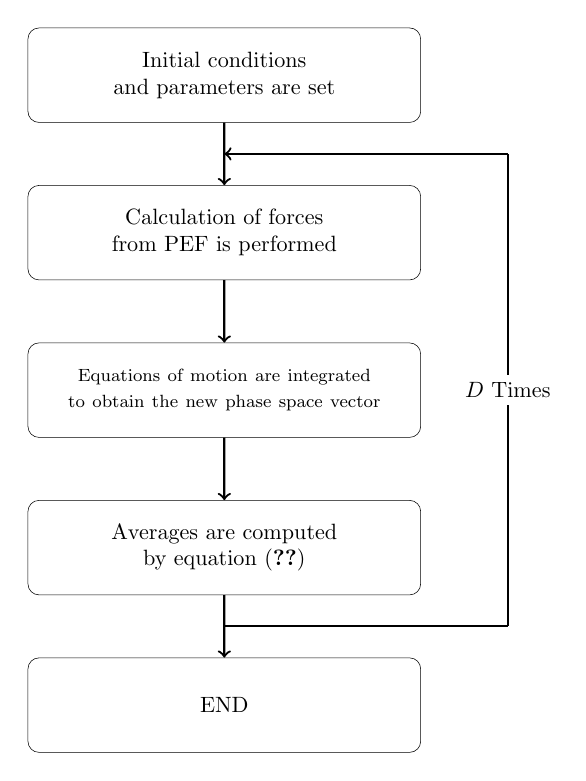
\begin{tikzpicture}[scale=0.8, transform shape]
	\node[rectangle,draw,rounded corners,very thin,minimum width=6cm,minimum height=1.5cm,text width=6cm,align=center] (A) at (0,10) {Initial conditions \\ and parameters are set};
	\node[rectangle,draw,rounded corners,very thin,minimum width=6cm,minimum height=1.5cm,text width=6cm,align=center] (B)  at (0,7.5) {Calculation of forces \\ from \ac{PEF} is performed};
	\node[rectangle,draw,rounded corners,very thin,minimum width=6cm,minimum height=1.5cm,text width=6cm,align=center] (C)  at (0,5) {\footnotesize Equations of motion are integrated to obtain the new phase space vector};
	\node[rectangle,draw,rounded corners,very thin,minimum width=6cm,minimum height=1.5cm,text width=6cm,align=center] (D)  at (0,2.5) {Averages are computed \\ by equation~(\ref{eq:MDTimeAve})};
	\node[rectangle,draw,rounded corners,very thin,minimum width=6cm,minimum height=1.5cm,text width=6cm,align=center] (E)  at (0,0) {END};
	\draw[thick,->] (A) -- (B);
	\draw[thick,->] (B) -- (C);
	\draw[thick,->] (C) -- (D);
	\draw[thick,->] (D) -- (E);
	\draw[thick,-] (0,1.25) -- (4.5,1.25);
	\draw[thick,-] (4.5,1.25) -- (4.5, 8.75) node[pos=0.5, fill=white] {$D$ Times};
	\draw[thick,->] (4.5, 8.75) -- (0, 8.75);
\end{tikzpicture}
\caption{Schematic representation of an \acs{MD} simulation.}
\label{fig:MDscheme}
\end{figure}

\subsection{Initial configuration}
In order to perform an \ac{MD} simulation it is necessary to select an \textit{initial configuration}. Its
choice can be nontrivial and it depends on the complexity of the system. Then, careful attention must be paid in
setting up the initial configuration.

Setting up an initial configuration means to prepare an $N$--particle system and assign all particle positions
and velocities, i.e. all the $6N$ coordinates of the initial phase space vector $\vec x(0)$. A common choice to
assign the initial velocities is to extract they randomly from the Maxwell--Boltzmann distribution function at a
specific system's temperature
\begin{equation*}
	f(v_i) = \sqrt{\frac{m_i}{2\pi k_B T}}e^{-\left ( \frac{m_iv_i^2}{2k_B T}\right )}
\end{equation*}
Moreover, the random assignment algorithm has to rescale all the velocities in such a way that the total system's
momentum $\vec P = \sum_{k=1}^N m_k\vec v_k$ is zero, this is equivalent to a \ac{COM} motion removal. This is
done because, in general, the total force acting on the system $\vec F = \sum_{k=1}^N \vec F_i$ is zero, then the
\ac{COM} motion is constant and to avoid a constant drift of the system in space this can be removed. Of course
this is a constraint on the system and it must be taken into account because it reduces the system \ac{DOF} by
three.

\subsection{Periodic boundary conditions}
In an \ac{MD} simulation the sample system is inserted into a \textit{simulation box} whose shape can be
differently chosen to better reproduce the symmetry of the simulated system. That box gives us the trivial
possibility to introduce a well defined reference system of coordinates. Obviously we must not forget to
correctly treat the \textit{boundary conditions}. In order to avoid surface effects and to consider only an
infinite bulk system, \ac{PBC} are imposed to the simulation box. This gives us also the possibility to simulate
system's bulk proprieties without considering a too large number of particles.
\begin{SCfigure}
	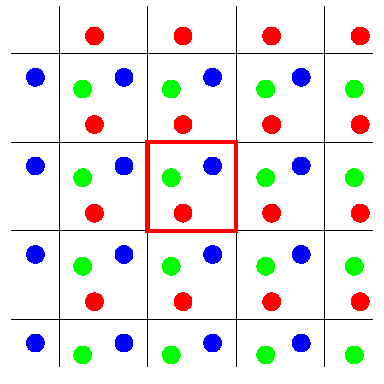
\includegraphics[width=0.4\textwidth]{./img/PBCScheme/PBCScheme}
	\caption{Schematic view of a two--dimensional box with \acs{PBC} imposed. The central, red contoured, box is the simulation box and it is replicated along each side.}
	\label{fig:pbc}
\end{SCfigure}
To give a better idea, in figure~(\ref{fig:pbc}) an example of a two--dimensional box with \ac{PBC} is shown. The
central red contoured box is the simulation box. The idea is to replicate that box in space along each side so
that there are no surface particles nor walls in the central box. When a particle moves in the central box, all
its images virtually move the same way in the copies of the box so that if a particle leaves the virtual boundary
of the central box, then, its nearest image enters the box and the number density of particles in the simulation
box is conserved. This virtual movement of image particles is achieved adjusting the positions of the simulation
box particles which have left the main box. For example, if one use a cubic box and a particle crosses its
boundary in one direction, say the $x$ direction, then its coordinate is corrected by subtracting (if it leaves
the box in the positive direction) or adding the box side length parallel to $x$ direction. Only box geometries
compatible with translational symmetry can be used. For example, nether a spherical nor a icosahedral box could
do the job. However when it is possible one have to use the most appropriate shape to better describe the
symmetry of the system, otherwise a closest approximation, compatible with \ac{PBC}, must be used.

Even if \ac{PBC} are used in a wide range of applications, it must be taken into account that imposing
periodicity to a system may affect its properties. A clear limitation of the periodic cell is that it is not
possible to achieve fluctuations that have a wavelength greater then the cell length. This cause, obviously, the
impossibility to sample those vibrating modes. Another problem arises with the range of the inter--particles
interactions: one have to choose carefully the size of the simulation box, or the number of particles if an $NPT$
ensemble is used, to ensure that the smallest simulation box length is greater then the interaction range. This
can be made easily for example with the Van der Waals interaction. On the contrary it is a difficult and time
consuming task to do the same with the electrostatic interactions that are treated with a more sophisticated
methods, as better explained in section~\ref{sec:longRangeInt}.

\subsection{Numerical integrators}
As we have seen above we need to solve numerically the equations of motion. Since the \ac{PEF} is a continuous
function of the phase space vector at a time $t$, the simplest way is to use the so called \textit{finite
difference} method. The basic idea is to expand the Newton's law in a Taylor series as follow
\begin{equation}
	\vec r_i(t + \delta t) = \vec r_i(t) + \vec v_i(t)\ \delta t + \frac{1}{2m_i}\vec f_i(t)\ (\delta t)^2\ +\ o((\delta t)^3)
	\label{eq:newtonTaylor}
\end{equation}
where we used the identities $\vec v_i(t) = \dot{\vec r}_i(t)$ and $m_i\ddot{\vec r}_i(t) = \vec f_i(t)$.

From this point, different algorithms have been developed. In the following we will describe in detail the most
important, the \textit{Verlet algorithm}, and its implementation the \textit{leap--frog algorithm}, which is the
default used in our \ac{MD} tools for this thesis work.

\subsubsection{Verlet algorithm}
The Verlet algorithm requires the positions and the forces at a time $t$ and the positions at a time $t-\delta t$
to calculate the positions at a time $t+\delta t$. Starting from equation~\eqref{eq:newtonTaylor} we can write
\begin{align}
	\vec r_i(t+\delta t) &\simeq \vec r_i(t) + \vec v_i(t)\delta t + \frac{1}{2m_i}\vec f_i(t)\ (\delta t)^2
	\label{eq:verlet1} \\
	\vec r_i(t-\delta t) &\simeq \vec r_i(t) - \vec v_i(t)\delta t + \frac{1}{2m_i}\vec f_i(t)\ (\delta t)^2
	\label{eq:verlet2}
\end{align}
from their sum we obtain the new positions at a time $t+\delta t$
\begin{equation}
	\vec r_i(t+\delta t) \simeq 2 \vec r_i(t) - \vec r_i (t - \delta t) + \frac{1}{m_i}\vec f_i(t)\ (\delta t)^2
	\label{eq:verletPosition}
\end{equation}
The velocities do not appear in the equation above and can be obtained taking the difference of
equation~\eqref{eq:verlet1} and~\eqref{eq:verlet2}
\begin{equation*}
	\vec v_i(t) \simeq \frac{\vec r_i(t+\delta t) - \vec r_i(t-\delta t)}{2\delta t}
\end{equation*}

Since positions in equation~\eqref{eq:verletPosition} are computed as differences this is a fourth order
algorithm and the precision is up to $o(\delta t)^4$, but they also contain a small term of order
$o(\delta t)^2$, ($\vec f_i(t)/(2m_i)$) which is summed to a difference of larger terms
($2 \vec r_i(t) - \vec r_i (t - \delta t)$). This may cause a loss of precision due to computer numerical representation.

The main disadvantage is that velocities at a time $t$ are an output of the calculation and not a part of the
algorithm itself. Moreover it is not self--starting because the algorithm required the positions at a time
$t-\delta t$. So at $t=0$ we need a trick to obtain the previous inexistent positions. The trick is to use
equation~\eqref{eq:verlet2} truncated at the first order: $\vec r_i(-\delta t) \simeq \vec r(0) - \vec v_i(0)\delta t$.

\subsubsection{Leap--Frog algorithm}
The leap--frog algorithm is a variant of the Verlet one and it is commonly implemented in many \ac{MD} tools, as
it is in our case. It computes the positions at a time $t$ and the velocities at a time
$t+\nicefrac{1}{2}\delta t$ from the forces at a time $t$ and the velocities at a time
$t-\nicefrac{1}{2}\delta t$. The main advantage with respect to the Verlet algorithm, is that it is
self--starting because it does not require the positions at a time $t-\delta t$.

First it calculates the velocities at a time $t+\nicefrac{1}{2}\delta t$ as follow
\begin{equation*}
	\vec v_i(t + \nicefrac{1}{2}\delta t) \simeq \vec v_i(t - \nicefrac{1}{2}\delta t) + \vec a_i(t)\delta t
\end{equation*}
then the positions at a time $t+\delta t$ are computed
\begin{equation*}
	\vec r_i(t + \delta t) \simeq \vec r_i(t) + \vec v_i(t + \nicefrac{1}{2}\delta t)\delta t
\end{equation*}
The velocities at a time $t$ can be calculated by
\begin{equation}
	\vec v_i(t) \simeq \frac{\vec v_i(t + \nicefrac{1}{2}\delta t) + \vec v_i(t - \nicefrac{1}{2}\delta t)}{2}
	\label{eq:lfVelocitiesSync}
\end{equation}

Another advantage is that the velocities are part of the algorithm itself and moreover it does not require the
calculation of the difference between two large numbers, with a gain of precision. The obvious disadvantage is
that the positions and velocities are not synchronized so the equation~\eqref{eq:lfVelocitiesSync} is necessary
to calculate the velocities at a time $t$. The need to have velocities at the same time of positions, as for the
Verlet algorithm, derives from the calculation of the kinetic energy contribution to the total energy: it must be
computed with positions and velocities at the same time.
%Discorso energia cinetica nello stesso tempo delle posizioni

\subsection{Neighbor list}
\label{sec:neighbor}
In order to solve the classical equations of motion, it is necessary to know the forces, and so the \ac{PEF},
acting on the system's particles. As we shall see in detail in the next section, this is one of the most time
consuming part of an \ac{MD} simulation. To know the forces acting on one particle, in principle, it is necessary
to calculate the contribution from all particles in the simulation box and all other periodic images. The most
popular way to speed up the simulation is to use a truncation of the interaction potentials within a cutoff. The
general idea is to compute the energy contribution of particle $i$ considering the interaction only with
particles $j$ that are closer to a certain cutoff distance $r_c$, thus such that
$\|\vec r_i - \vec r_j\| \le r_c$. This is summarized in the following expressions
\begin{equation*}
	U_i(\vec r) = \sum_{j\ne i}^N U^*_{ij}(\vec r), \qquad U^*_{ij}(\vec r) = \left \{
	\begin{aligned}
		& U_{ij}(\vec r)& \qquad  &\| \vec r_i - \vec r_j \| \le r_c \\
		& 0			    & \qquad  &\text{otherwise}
	\end{aligned}
	\right .
\end{equation*}
where $U_{ij}(\vec r)$ is the interaction potential between particles $i$ and $j$.

By itself, the use of a truncation of the potential may not dramatically reduce the time spent in computing the
inter--particle interactions. This is because, in order to decide for what particles we have to compute the
interactions, we have to compute the distances between every pair of particles in the system. A marked increase
of performance is achieved by the use of a \textit{neighbor pair--list}. The simplest way is to consider, for
each particle, a list of its neighbor particles that lie within a sphere of radius $r_c$ surrounding the selected
particle. Then, for each particle, the interactions are computed between the selected particle and those that are
in its pair--list. There is a gain in performance if the pair--list is updated at least every $M>1$ \ac{MD}
steps. This is possible taking into account that, typically, in \ac{MD} simulations of liquids system at ambient
temperature and pressure, a particle neighbors do not change significantly for $M < 20$ time steps.

Anyway particles move during the non--updating time so that some of them may cross the pair--list causing an
over-- or under--estimation of the inter--particle energy contribution. To partially solve this problem, as
suggested by Verlet \cite{VerletList}, one can consider a \textit{buffered} pair--list or a \textit{Verlet
cut--off scheme} in which the pair--list is constructed considering those particles that are close to the
selected one by a distance of $r_l > r_c$, called \textit{list radius}. That pair--list is updated every some
time steps, but every time steps the pairwise contribution is computed only between those particles in the
pair--list for which the distance is less then $r_c$. Thus, at the cost of slightly decrease the performance
compared to the un--buffered pair--list, almost none of the interacting particles within the cutoff is neglected.
Nevertheless, since a too big list radius and a too small list update frequency leads to a loss of performance,
particle--pairs could still move enough during the non--updating time and have a chance to cross the boundary of
the buffered pair--list $r_l$. This chance leads to a small energy drift proportional to the system temperature.
In simulations with a constant temperature coupling, i.e. in a canonical or isothermal--isobaric ensemble, the
extra radius of the buffered pair--list can be dynamically determined, during the simulation, by fixing an upper
limit to the energy drift. That tolerance is often called \textit{Verlet buffer tolerance}. In
figure~(\ref{fig:pairlist}) a schematic representation of the buffered pair--list construction is shown.
\begin{SCfigure}
	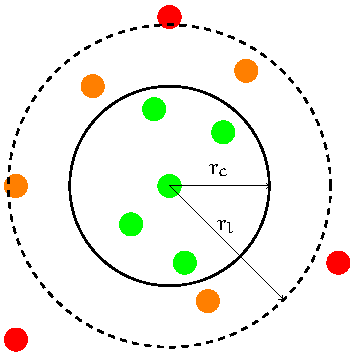
\includegraphics[width=0.42\textwidth]{./img/pairList/pairList}
	\caption{Schematic representation of the buffered pair--list construction respect to the central particle.
	Green particles are in the pair--list below the cutoff radius $r_c$, therefore included in the calculation of the interactions. Orange particles are in the pair--list for which at every step is checked if their distances became smaller then $r_c$. Red particles are not in the pair--list and they are completely neglected until the next list update.}
	\label{fig:pairlist}
\end{SCfigure}

A better performance can be achieved adding a dynamic update algorithm of the pair--list refresh rate during the
simulation. A nice way is to consider the maximum distance traveled by a particle in the pair--list: if this
distance is greater than $r_b = r_l - r_c$ then the pair--list is certainly updated. Thus one can fix the refresh
rate to a higher value increasing the performance.

\subsection{Thermostat algorithms} %Molecular Modelling, 382
A thermostat is an external tool that allows to maintain a system at a constant temperature. Several algorithms
are available. Some are based acting on particle velocities (Anderson, Berendsen, Bussi) other introduce some
more \ac{DOF} in the system that take into account a real temperature bath coupling (Nosé--Hoover). We will
describe in more detail the one used in this thesis work.

As suggested by Bussi \etal\, \cite{Bussi}, a common practice to implement a thermostat acting on particle
velocities is related to a \textit{velocity rescale} algorithm in which the velocities of all particles are
scaled by some factor. The simplest way is to consider the total kinetic energy $K$ of the system as in
equation~\eqref{eq:kinetic} and the average kinetic energy $\ave{K}$ obtained from equation~\eqref{eq:kineticT}
with the substitution $3N\rightarrow N_f$
\begin{equation*}
	\ave{K} = \frac{1}{2}N_f k_B T
\end{equation*}
where $N_f$ is the \textit{total} \ac{DOF} of the system and $T$ is the target temperature. Thus the scaling
factor is defined by
\begin{equation*}
	\alpha_{T} \equiv \sqrt{\frac{\ave{K}}{K}}
\end{equation*}

The scaling operation is usually performed at a fixed rate during the simulation, or when the kinetic energy
exceeds the limits of an interval centered around the target value. However the sampled ensemble is not
explicitly known but, since in the thermodynamic limit the average properties do not depend on the ensemble
chosen, even this very simple algorithm, often called \textit{weak coupling thermostat}, can be used to produce
useful results. Despite this, for small systems or when the observables of interest are dependent on the
fluctuations rather than on the averages or when other methods assume a canonical sampling, this method cannot be
safely used.

In order to obtain the correct canonical sampling Bussi \etal\, \cite{Bussi} modify the way to calculate
$\alpha_T$ so as to enforce a canonical distribution for the kinetic energy. The new scaling factor is obtained
from
\begin{equation*}
	\alpha_{T} \equiv \sqrt{\frac{K_T}{K}}
\end{equation*}
where $K_T$ is extracted with a stochastic procedure from the equilibrium canonical distribution of the kinetic
energy, given by
\begin{equation*}
	P(K_T)dK_T \propto K_T^{N_f/2-1}\ e^{-\beta K_T}\ dK_T
\end{equation*}
where $P(K_T)dK_T$ is probability that the system has a kinetic energy between $K_T$ and $K_T + dK_T$.

Since velocities are scaled only after some \ac{MD} steps this can cause a discontinuity in the particle
velocities just before and after the scaling step. To avoid this problem, the authors suggest that the choice of
$K_T$ can be based on the previous value of $K$ so as to obtain a smoother evolution. The procedure proposed by
Bussi \etal\, consists in the following steps
\begin{itemize}
	\item Evolve the system for a single time step solving the equations of motion, so as to be in an $NVE$ ensemble;
	\item Calculate the total kinetic energy and evolve it for a single time step using an auxiliary continuous stochastic dynamics;
	\item Rescale the velocities by $\alpha_T$ so as to enforce this new value of the kinetic energy.
\end{itemize}

The authors have shown that an auxiliary dynamics for the kinetic energy of the form
\begin{equation*}
	dK = \frac{\ave{K} - K}{\tau_T}\ dt + 2 \sqrt{\frac{K\ave{K}}{N_f\tau_T}}\ dW
\end{equation*}
can do the job. Where $dW$ is a Wiener stochastic noise and $\tau_T$ is an arbitrary parameter which is related
to the response time of the thermostat. In fact it reduces to the simple week coupling rescale if
$\tau_T\rightarrow 0$ and to the Hamiltonian dynamics (as an $NVE$ ensemble) if $\tau_T\rightarrow +\infty$.
Until the system is at non--equilibrium the first deterministic part is dominant an drives the system to
equilibrium with a characteristic time $\tau_T$. Then the stochastic contribution samples the canonical
distribution.


\subsection{Barostat algorithms} %Molecular Modelling, 382
As the thermostat maintains the system at a constant temperature $T$, a barostat is needed to maintain the system
at a constant pressure $p$. To do this the system is coupled to a sort of piston so that changing the volume of
the simulation box will adjust the pressure.

\subsubsection{Berendsen algorithm}
A common way, as proposed by Berendsen, is to scale both volume and particle coordinates. The rate of change of
the pressure is given by
\begin{equation*}
	\frac{dp}{dt} = \frac{p_0 - p}{\tau_p}
\end{equation*}
where $p_0$ is the target pressure, $p$ is the instantaneous system pressure given by
equation~\eqref{eq:pressure} and $\tau_p$ is a coupling constant related to the response time of the barostat.
Thus if we consider a time step $\delta t$ then the volume scaling factor $\lambda$ is given by
\begin{equation*}
	\lambda = 1- k_T (p_0 - p) \frac{\delta t}{\tau_p}
\end{equation*}
where $k_t$ is the isothermal compressibility defined as
\begin{equation*}
	k_T = -\frac{1}{V}\left ( \frac{\partial V}{\partial p}\right )_{T}
\end{equation*}
while the factor $\nicefrac{\delta t}{\tau_p}$ gives a scaling factor for the isothermal compressibility that
allow us to take into account the finite response time of the barostat. If $\tau_p \rightarrow 0$ the system has
an infinity isothermal compressibility so it is necessary a really small change in volume to achieve the correct
pressure; on the contrary if $\tau_p \rightarrow +\infty$ the system reduces to the Hamiltonian
dynamics\footnote{If the system is coupled to a thermostat, then the canonical ensemble is sampled.}. The
particle coordinates is scaled by the factor $\lambda^{\nicefrac{1}{3}}$.

In the case of anisotropic system the pressure matrix $\mathbold{P}$ and the volume matrix $\mathbold{H}$
\eqref{eq:volumeMatrix} have to be considered and the Berendsen algorithm can be generalized such that even
$\lambda$ becomes a $3\times 3$ matrix. However the main problem, as for the weak coupling thermostat, is that
the sampled ensemble is not known. Thus a new approach, in order to correct sample the isobaric ensemble, has
been derived by Parrinello and Rahman.

\subsubsection{Parrinello--Rahman algorithm}
The Parrinello--Rahman barostat \cite{ParrinelloBarostat1}\cite{ParrinelloBarostat2} is based on genuinely treat
the coupling of the system to an external piston of ``mass'' $M_h$ through a Lagrangian method in which the
volume becomes a Lagrangian variable of the system and its time evolution can be computed solving the
Euler--Lagrange equations. Both the size and the shape of the simulation box are allowed to fluctuate. So it is
perfectly compatible with anisotropic system. The shape and size of the simulation box are described by the
volume matrix $ \mathbold{H}$ in equation~\eqref{eq:volumeMatrix} such that $V = |\det\mathbold{H}|$.
$\mathbold{H}$ is the Lagrangian coordinate of the external piston. If the external pressure $p_0$ is applied to
the piston then its potential energy is given by
\begin{equation*}
	U_p = p_0 |\det  \mathbold{H}|
\end{equation*}
instead, if $ \mathbold{H}$ varies in time then a ``kinetic energy'' is associated to the piston as follow
\begin{equation*}
	K_p = \frac{1}{2}M_h \text{Tr}(\leftidx{^t}{\dot{ \mathbold{H}}}{} \dot{ \mathbold{H}} )
\end{equation*}
where $\leftidx{^t}{(\cdot)}{}$ denote the transpose operation.

In order to write the Lagrangian of the system the particle coordinates must be expressed in terms of
$\mathbold{H}$. This can be done defining the vector $\vec s_i$ so that $\vec r_i =  \mathbold{H} \vec s_i$. The
square displacement can be obtained as $\vec r_i \cdot \vec r_i = \leftidx{^t}{ (\mathbold{H} \vec s_i)}{}  \mathbold{H} \vec s_i = \leftidx{^t}{\vec s_i}{} \leftidx{^t}{ \mathbold{H}}{}  \mathbold{H} \vec s_i$, often
$\mathbold{G} = \leftidx{^t}{ \mathbold{H}}{} \mathbold{H}$. Parrinello \etal\, write the Lagrangian as follow
\begin{equation*}
	\mathcal{L} = \frac{1}{2}\sum_{i=1}^N m_i \dot{\vec s}_i \leftidx{^t}{\mathbold{G}}{} \dot{\vec s}_i - \sum_{i=1}^N \sum_{j=i+1}^N U_{ij}(\vec r) +  \frac{1}{2} M_h \text{Tr}(\leftidx{^t}{\mathbold{\dot H}}{} \mathbold{\dot H} ) -  p_0 |\det \mathbold{H}|
\end{equation*}
thus the equations of motion for $ \mathbold{H}$ and $\vec s_i$ can be computed solving the Euler--Lagrange
equations. It can be shown that the equations of motion, derived in \cite{ParrinelloBarostat1} and
\cite{ParrinelloBarostat2}, correct sample an isobaric ensemble. A practical way to show it, is to consider the
Hamiltonian of the system. Using equation~\eqref{eq:hamiltonian} the Hamiltonian is
\begin{equation*}
	\mathcal{H} = \frac{1}{2}\sum_{i=1}^N m_i \dot{\vec s}_i \leftidx{^t}{\mathbold{G}}{} \dot{\vec s}_i + \sum_{i=1}^N \sum_{j=i+1}^N U_{ij}(\vec r) +  \frac{1}{2} M_h \text{Tr}( \leftidx{^t}{\mathbold{\dot H}}{} \mathbold{\dot H} ) + p_0 |\det\mathbold{H}|
\end{equation*}
if the system is in equilibrium at temperature $T$, using the equipartition theorem, the kinetic term of the
system particles contributes to the energy by $3Nk_BT/2$ while the kinetic term of the piston by $9k_BT/2$. Since
$3N \gg 9$ the Hamiltonian can be approximated by
\begin{equation*}
	\mathcal{H} \simeq \ave{K} + U + p_0 V = H
\end{equation*}
that is the enthalpy. Since the Hamiltonian is a constant of motion the correct isobaric ensemble is sampled. If
the system is also coupled to a thermostat, the $-TS$ term must be added, so the constant of motion become the
Gibbs free energy $G = H - TS$ and the isobaric--isotherm ensemble is correctly sampled.

In order to understand the meaning of the $M_h$ parameter (the piston ``mass'') we report the dynamic equation of $\mathbold H$
\begin{equation*}
	M_h \mathbold{\ddot H} = V (p - p_0) (\leftidx{^t}{\mathbold{H}}{})^{-1}
\end{equation*}
The Parrinello--Rahman barostat is like a second order system. When there is an imbalance between the
instantaneous internal pressure $p$ (see equation~\eqref{eq:pressure}) and the target pressure $p_0$, the system
recovers this imbalance in a characteristic time governed by the parameter $M_h$. Since at equilibrium the
properties of a system are independent of the masses of its constituent parts, $M_h$ can be arbitrarily chosen if
one is interested only in static averages, otherwise a more appropriate choice must be made to obtain accurate
dynamical properties. In this case, the authors suggest a choice of $M_h$ such that the relaxation time is of the
order of $L/c$ where $L$ is simulation box size and $c$ is the sound velocity.

Interesting is the fact that this algorithm can be generalized to an anisotropic pressure coupling making use of
the theory of elasticity. Differently from the Berendsen algorithm, Parrinello--Rahman method is much slower in
changing the volume until the equilibrium value is reached and it is less stable: if the system is not well
equilibrated can lead to a large volume fluctuation with can compromise the simulation success. On the other hand
the Parrinello--Rahman samples correctly the isobaric ensemble. A common strategy is to use the Berendsen
barostat to reach equilibrium then switch to the Parrinello--Rahman algorithm to correctly sample the phase space
associated to the isobaric ensemble.

\newpage
\section{Advanced sampling methods}
The free energy is a quantity of particular importance for the equilibrium statistical mechanics. The 
Gibbs free energy $G$ is specific for the $NPT$ isobaric--isothermal ensemble and the Helmholtz free energy $A$ 
for the $NVE$ canonical ensemble. The time evolution of a biomolecular system and its equilibrium properties are 
determined by the system's \ac{FES}. This because free energy differences tell us, for example, if a chemical 
reaction occurs spontaneously, whether a given solute is hydrophobic or hydrophilic, if a protein conformational 
change can take place or whether some molecules in water solution are able to self--assemble into a more complex 
system and so forth. Being related to the partition function of an ensemble, the free energy is the generator 
through which other thermodynamic quantities are obtained via differentiation. However often we are particularly 
interested in the free energy difference between two thermodynamic states, instead of the absolute value. 

\paragraph{\textbf{Collective variables}} Often, we are interested in the \ac{FES} in function of some
generalized coordinates, called \acp{CV} of the system. These small set of variables can describe, in a simple
and useful manner, some chemical, thermodynamic or mechanical processes that take place in the system. For
example, the free energy in function of the distance between the \ac{COM} of two molecules give us information
about their attraction or repulsion and if they form a bound state. Thus the \ac{FES}, in the \acp{CV} space,
provides a map of the stable conformations, the relative stability of these conformations and the barrier heights
that must be crossed for the transition to take place. Moreover, the energy landscape, even for a small molecule,
can be extremely wrinkled and the large number of minima can not be sampled in a typical \ac{MD} simulation. The
principal reason for the use of the \acp{CV}, is thus to limit the sampling to those regions of phase space that
are most important for the process under study, hoping that the limited sampled regions are sufficient to
correctly describe the process.
%It is necessary to stress out that in many cases one do not know exactly \textit{a priori} the \ac{FES} about a certain process and so one want to know it also for understand if other minima energy configurations exist, in addition to those known, how stable they are and what are the energy barriers to go from one minima state to an other\footnote{Sometimes thought the cinematic of an \ac{MD} simulation one can gamble an estimate of the functional form of the \ac{FES}, looking for the relative probability to stay in a meta--stable state rather then the other. Clearly this means that both meta--stable states are to be sampled, as we shall see later it depends of the height of the energy barriers.}.

\paragraph{\textbf{Free energy surface}} The calculation of free energy difference between two thermodynamic
states (that requires an \textit{a priori} knowledge of the two stable states) and the calculation of the
\ac{FES} are one of the main challenges in \ac{MD} simulations for biomolecular applications. Let us suppose that
we are interested in the \ac{FES} in function of the \ac{CV} $s(\vec r)$ and we are working in a $NPT$
ensemble\footnote{The following is still valid even for a $NVE$ ensemble with the substitution $G\rightarrow A$
and the use of the correct partition function $\mathcal{Z}_{NVE}$.} with an isotropic system. Following
section~\ref{sec:statmec}, the Gibbs free energy along the \ac{CV} is obtained as
\begin{equation}
	G(s) = -k_BT \ln Q(s)
	\label{eq:fes}
\end{equation}
where $Q(s)$ is the partition function that integrate out all the \ac{DOF} of the system expect for $s(\vec r)$:
\begin{equation*}
	Q(s) = \frac{1}{\mathcal{Z}_{NpT}} \int_0^{+\infty}\ dV \ \int_\Omega e^{-\beta(\mathcal{H}(\vec x) + pV)}\delta(s(\vec r) - s)\ dx
\end{equation*}
since $s(\vec r)$ does not depend on particle momenta, from equations~\eqref{eq:hamiltonian}
and~\eqref{eq:nptPartition}, $Q(s)$ can be rewritten as
\begin{equation}
	Q(s) =  \frac{ \int_\Omega e^{-\beta U(\vec r)}\delta(s(\vec r) - s)\ dr }{\int_\Omega e^{-\beta U(\vec r)}\ dr}
	\label{eq:CVprobability}
\end{equation}
where $U(\vec r)$ is the \ac{PEF}. $Q(s)ds$ can be interpreted as the probability to find the system with
$s(\vec x)$ between $s$ and $s + ds$. Since this equation contains a direct phase space integration it can be
rewritten in a more useful manner using the ensemble averages and then, using the ergodic theorem in
equation~\eqref{eq:ergotic}, as a time average:
\begin{equation}
	Q(s) = \ave{\delta(s(\vec r) - s)} = \lim_{t\to +\infty}\frac{1}{\tau}\int_0^\tau \delta(s(\vec r(t)) - s)\ dt
	\label{eq:CVprobabilityAve}
\end{equation}

The time sampling of equation~\eqref{eq:CVprobabilityAve} can be
derived, in principle, via \ac{MD}. Unfortunately, since the time can not be infinite, the main problem related
to \ac{MD} simulations is whether we are able to correctly sample \textit{all} the phase space of an ensemble in
order to compute the ensemble average. Clearly the answer depends on the system in exam, if it is really simple
maybe we can do that, otherwise probably not or indeed it take too much time and/or we are not able to collect
sufficient data. This sampling problem can be summarized as follows: regions in phase space around a local
minimum of the \ac{FES} are typically sampled well, whereas regions of higher energy are sampled rarely. These
high energy regions provide with a small contribution to the partition function, due to their unfavorable
Boltzmann factor. However they must be overcome in order to sample other minima that can give, instead, a
important contribution to the ensemble averages. These transitions are called \textit{rare events}. When the
system is moving in the energy landscape the only way to escape from a local minimum is to exploit thermal
fluctuations and so energy barriers that are higher then $\sim k_B T$ have a small probability of being overcome.

\paragraph{\textbf{Bias based advanced sampling}} Several methods are developed and are still in development in
order to solve the just described sampling problem. These methods are all based on advanced sampling techniques
that allow us to
\begin{itemize}
	\item Escape from a local energy minimum, in order to explore other regions of the phase space;
	\item Calculate the free energy difference between two thermodynamic states;
	\item Compute the \ac{FES} along one or a small set of \acp{CV}.
\end{itemize}
The common basic idea is to introduce a additional \textit{bias potential} able to confine the sampling to a
limited region of the \ac{CV} space and/or drive the transition between two metastable configuration. In
particular we describe only those methods used in this thesis work: \textit{umbrella sampling method} and
\textit{metadynamics}. For a more comprehensive discussion the reader is addressed to the review by Kästner
\cite{Umbrella} for the former, and to the review by Laio and Gervasio \cite{MetadReview} for the latter.
Moreover in the books by Tuckerman \cite{Tuckerman} other enhanced sampling methods are described.

\subsection{Umbrella sampling}
The umbrella sampling method was developed by Torrie and Valleau and today is one of the most mature and broadly
accepted method for calculating free energy differences. The basic idea is to drive the system from a known state
$A$ to an other known state $B$ through a deterministic path defined on the \ac{CV} $s(\vec r)$ chosen to
describe the process. This method is well suited for one \ac{CV}, otherwise the computational performance
degrades rapidly with the number of \acp{CV}. The idea is to identify a path connecting $A$ to $B$, and divide it
into a discrete number of windows $N_w$ and take a subset $\{s_i\}$, $i=1,\dots,N_w$ of the values assumed by the
continuos \ac{CV} from state $A$ to $B$ along the path. For each of these target values $s_i$ a bias potential
$w_i(s)$, depending only on $s$, is added to \ac{PEF} in order to restrain the system to the $s_i$ target value.
Then, \ac{MD} simulations are performed for each window. All the data collected within the $N_w$ windows are
combined together to compute the biased \ac{FES} along the chosen \ac{CV}. Eventually, the unbiased \ac{FES} is
recovered. In figure~(\ref{fig:umbrellaPath}) an example of the windows selection is shown.
\begin{SCfigure}
	\centering
	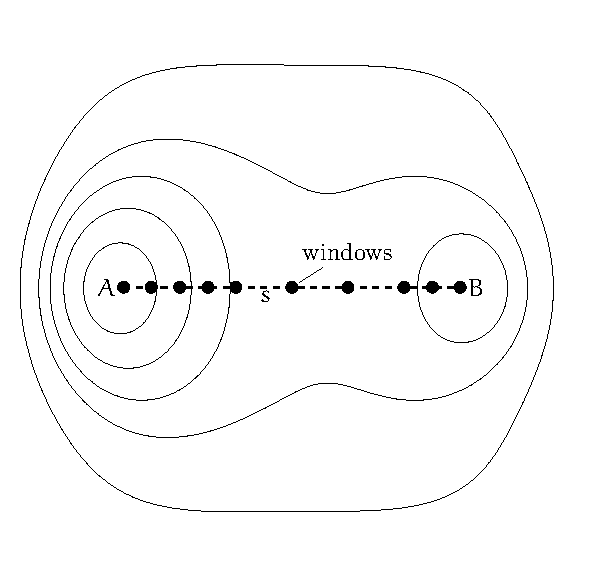
\includegraphics[width=0.45\textwidth]{./img/umbrellaPath/umbrellaPath.pdf}
	\caption{Example of an umbrella sampling windows selection. The contour plot represent a $2$--minima free energy profile through which the system is evolved. The dashed line is the path along the \acs{CV} $s(\vec r)$ that connect state $A$ to $B$. The black filled circles represent the selected windows for different values of $s$.}
	\label{fig:umbrellaPath}
\end{SCfigure}

Suppose $w_i(s)$ to be the bias potential applied on window $i$ in function of the \ac{CV} $s(\vec r)$. Then the
biased \ac{PEF} of window $i$ become $U_i^b(\vec r) = U(\vec r) + w_i(s)$; where the superscript $b$ denotes
biased quantities. With the substitution $U(\vec r) \rightarrow U_i^b(\vec r)$ in
equation~\eqref{eq:CVprobability} the corresponding biased partition function integrated over all \ac{DOF} but
$s$ yields to
\begin{equation*}
	Q_i^b(s) = e^{\beta w_i(s)}\frac{ \int_\Omega e^{-\beta U(\vec r)}\delta(s(\vec r) - s)\ dr }{\int_\Omega e^{-\beta (U(\vec r) + w_i(s(\vec r)))}\ dr}
\end{equation*}
In order to use equation~\eqref{eq:fes} to obtain the \ac{FES}, we need to recover the un--biased partition
faction $Q_i(s)$ like in equation~\eqref{eq:CVprobability}. This can be done (see \cite{Umbrella}), obtaining the
following expression
\begin{equation}
	\begin{aligned}
	Q_i(s) &= Q_i^b(s) e^{\beta w_i(s)}\ \frac{ \int_\Omega e^{-\beta U(\vec r)}e^{-\beta w_i(s(\vec r))}\ dr }{\int_\Omega e^{-\beta U(\vec r)}\ dr} = \\
		   &= Q_i^b(s) e^{\beta w_i(s)}\ \ave{e^{-\beta w_i(s)}}
	\end{aligned}
	\label{eq:windowPartFunc}
\end{equation}
then the \ac{FES} for window $i$ is obtained simply by equation~\eqref{eq:fes}
\begin{equation*}
	G_i(s) = -k_BT \ln Q_i^b(s) - w_i(s) + C_i
\end{equation*}
where $Q_i^b(s)$ is obtained as an ensemble average via the biased \ac{MD} simulation like
equation~\eqref{eq:CVprobabilityAve} and $w_i(s)$ is a known function. $C_i$ is an addictive constant independent
of $s$ that connects the free energy curves $G_i(s)$ of different windows. As we shall see, in order to combine
more windows to calculate a global \ac{FES}, all $\{C_i\}$ must be computed.

\paragraph{\textbf{Weighted histogram analysis method}} Different analysis methods have been developed in order
combine informations collected from the $N_w$ windows. The aim of those methods is to compute the global unbiased
partition function $Q(s)$ from the set of biased partition functions $\{Q^n_i(s)\}$ in order to extract the
global \ac{FES} $G(s)$. The most commonly used method is the \ac{WHAM} \cite{WHAM}, \cite{gWHAM}. The philosophy
behind it is to minimize the statistical error in the calculation of $Q(s)$. For each of the $N_w$ biased windows
a set of histograms $\{h_i(s)\}$ with $n_i$ bins, representing the set $\{Q^b_i(s)\}$, is recorded. The global
distribution function is computed as follow
\begin{equation}
	Q(s) = \sum_{i=0}^{N_w} p_i h_i(s), \qquad \sum_{i=0}^{N_w} p_i = 1
	\label{eq:whan1}
\end{equation}
where $p_i$ are weights chosen to minimize statistical error on $Q(s)$. Those leads to
\begin{equation}
	p_i = \frac{n_ie^{-\beta (w_i(s) - C_i)}}{\sum_{j=0}^{N_w} n_je^{-\beta (w_j(s) - C_j)}}
	\label{eq:whanwheight}
\end{equation}
where $n_i$ is the total number of independent bins in the $i-$th histogram. The problem now is to compute the
set of constants $\{C_i\}$. We can not use the integrals in equation~\eqref{eq:windowPartFunc} for the problems
already described at the begging of this section, but the second line give us an idea. The ensemble average can
be computed using the global distribution function $Q(s)$ as follow
\begin{equation}
	e^{-\beta C_i} = \ave{e^{-\beta w_i(s)}} = \int Q(s) e^{-\beta w_i(s)}\ ds
	\label{eq:whan2}
\end{equation}
Because $Q(s)$ in equation~\eqref{eq:whan1} depends on the set of constants $\{C_i\}$ and \textit{vice versa},
both equations must be solved in a iterative self--consistent manner. A first guess of set $\{C_i\}$ is used to
compute the weights from equation~\eqref{eq:whanwheight} then from equation~\eqref{eq:whan1} $Q(s)$ is computed
and it is used to obtain a new set of constants $\{C_i\}$ from equation~\eqref{eq:whan2} and so on until both
equations are satisfied. When the iteration procedure is completed the global \ac{FES} $G(s)$ is obtained from
equation~\eqref{eq:fes}. One important consideration about \ac{WHAM} is that the histograms in adjacent windows
must be sufficiently overlapped otherwise the statistical error due to the combining procedure can be too high or
the iterative procedure itself can lead to convergence problems.

\paragraph{\textbf{Bias potential}} The bias potential is chosen such that sampling along the \ac{CV} is uniform.
Together with \ac{WHAM} a simple harmonic bias potential is most commonly used for its simplicity. In order to
restrain the system to the target value $s_i$ of the \ac{CV} $s(\vec r)$ along the path chosen to connect state
$A$ and $B$, each window is biased with a harmonic potential of the form
\begin{equation*}
	w_i(s) = \frac{1}{2}K (s - s_i)^2
\end{equation*}
The choice of $K$, the strength of the bias potential, is a critical point. $K$ has to be large enough to
appropriately sample the corresponding modes. However too large $K$ cause too narrow distributions that can cause
overlap problems, hence the necessity for $K$ to be as small as possible to allow for some overlap between
windows.

%\paragraph{\textbf{error estimation}}

\bigskip The implementation of the umbrella sampling method can be summarized in the following procedure
\begin{itemize}
	\item A \ac{CV} that well describes the transition process from state $A$ to $B$ and a connecting path are chosen;
	\item A subset of the values assumed by the \ac{CV} along the path are taken and for each a biased \ac{MD} simulation is performed\footnote{Since each biased simulation is independent they can be performed in parallel with the other.};
	\item Using \ac{WHAM} the set of biased partition functions $\{Q^b_i(s)\}$ are combined in order to compute the global unbiased partition function $Q(s)$. Then $G(s)$ is calculated.
\end{itemize}


\subsection{Metadynamics}
\label{sec:metadynamics}
The metadynamics method was originally developed by Parrinello and Laio \cite{MetadParrinello} with the first aim
to accelerate the escaping from a free energy minimum in \ac{MD} simulations. The success of the method soon led
to the creation of a unified framework for accelerating rare events and computing free energies in function of a
small set of \acp{CV}. The main advantages with respect to umbrella sampling method is that several \acp{CV},
instead of a single one, can be simultaneously used without affecting the simulation performance. The basic idea
of metadynamics is to enhance the dynamics of a system along some \acp{CV} simply by filling the corresponding
energy minimum with an history--dependent bias potential, in order to sample larger and larger portions of the
phase space. Supposing a two state process from state $A$ to $B$, in the \ac{CV} space, if the deposited energy
is sufficient to fill the energy well of state $A$, the system is favorably disposed to overcome the barrier and 
go to the state $B$. In figure~(\ref{fig:fancyMetadyn}) a simple scheme of that cartoon is shown. 
\begin{SCfigure}[][hb]
	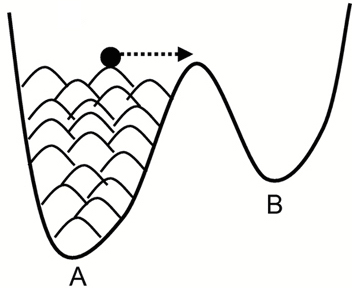
\includegraphics[width=0.35\textwidth]{./img/fancyMetadyn}
	\caption{Schematic cartoon of the energy well filling by the history--dependent bias potential and the consequently transition from state $A$ to state $B$.}
	\label{fig:fancyMetadyn}
\end{SCfigure}

This novel idea is supported by the assumption of Parrinello and Laio, based on experimental and heuristic 
results, that iteratively summing the deposited potential during the biased \ac{MD} simulation leads to
an estimator of the \ac{FES} along the chosen \acp{CV} in the region explored. If
$\vec s(\vec r) = (s_1(\vec r), \cdots, s_n(\vec r))$ is the \acp{CV} vector, where $n$ is a small number, and
$w(\vec s, t)$ is the bias potential deposited every $\tau$ \ac{MD} time steps the ``metadynamics''
history--dependent potential acting on the system at a time $t$ is given by
\begin{equation*}
	w_M(\vec s, t) = \sum_{\substack{i=0 \\ i\tau < t}} w(\vec s, i\tau)
\end{equation*}
where $t$ is the time in unit of \ac{MD} time step. The time dependence in the bias potential $w(\vec s, t)$ is
needed since it has to depend on the values assumed by the \acp{CV} at some previous \ac{MD} steps. The 
Parrinello and Laio assumption yields to the following expression
\begin{equation}
	\lim_{t\to + \infty} w_M(\vec s, t)  \simeq -G(\vec s) + C
	\label{eq:metadfes}
\end{equation}
where $C$ is an addictive constant. Since the history--dependent potential iteratively compensates the underlying
\ac{FES}, the system evolved with metadynamics \textit{tends to escape from any energy minima via the lowest
saddle point}. Thus, to the contrary of umbrella sampling metadynamics is suitable, not only to compute
efficiently \ac{FES}, but also to explore new reaction path and accelerate the observation of rare events. If the
\acp{CV} are chosen sensibly the system will quickly find its way over the lowest free energy saddle point and
evolve over the next minimum as it would do in a \textit{very long} \ac{MD} simulation.

A possible bias potential can be deduced considering equation~\eqref{eq:CVprobabilityAve}. The Dirac delta
function can be expressed by its approximant:
\begin{equation*}
	\delta(x-a) = \lim_{\sigma\to 0}\ \frac{1}{\sqrt{2 \pi \sigma^2}}e^{-(x-a)^2/(2\sigma^2)}
\end{equation*}
then substituting in equation~\eqref{eq:CVprobabilityAve} we have
\begin{equation*}
	Q(s) = \frac{1}{\sqrt{2\pi}}\lim_{t\to +\infty}\ \lim_{\sigma\to 0} \frac{1}{\sigma t}\int_0^t \exp{ \left ( -\frac{(s(\vec r(\tau))-s)^2}{2\sigma^2} \right )} \ d\tau
\end{equation*}
the equation above suggests the use of a Gaussian function centered around the values assumed by the \ac{CV} at a
time $t$. Then the bias potential component, extended to multiple \acp{CV}, is chosen as follow
\begin{equation*}
	w(\vec s, t) = w\ \exp\left ({-\sum_{i=0}^n \frac{(s_i - s_i(\vec r(t)))^2}{2{\delta s_i}^2} }\right )
\end{equation*}
where $w$ is the height and $\delta s_i$ is the width of the deposited Gaussians.

For setting up a metadynamics simulation, there are three parameters to choose carefully: the height $w$ and the
width $\delta s_i$ of the deposited Gaussians and the stride of deposition $\tau$. All these parameters affect
the accuracy and the efficiency of the free energy profile reconstruction. Clearly if the Gaussians are big and
large or placed too quickly the \ac{FES} will be explored at a fast pace but the reconstructed profile will be
affected by large errors. Instead if they are small or placed infrequently the reconstruction will be accurate
but will take a longer time. Moreover the time required to escape from a local minimum is determined by the
number of Gaussians necessary to fill the well. This number is proportional to $(1/\delta s)^n$
\cite{MetadReview}, hence the necessity to maintain the number $n$ of \acp{CV} as small as possible or increase
the Gaussian width. On the other hand the history--dependent potential can only reproduce features of the
\ac{FES} on a scale larger then $\sim \delta s$. Empirical criteria can be used to choose the $\delta s$ and
$\tau$ parameters; the former by monitoring the standard deviation of the \acp{CV} in an unbiased \ac{MD}
simulation and the latter by considering the relaxation time of the system after a Gaussian is deposited: clearly
the bigger is the Gaussian the more time is needed by the system to relax. However it does not exist an universal
and general recipe to choose these parameters, only some knowledge of the system and process under study can give
useful hints. They can certainly be fine tuned in successive steps.

In figure~(\ref{fig:metadEs}) an example of the time evolution of a metadynamics simulation is shown. We can see
that as the number of deposited Gaussians increases the system is able to visit more regions of the phase space.
Moreover, as the simulation time increases, when the energy landscape (lower panel) becomes flat the system
becomes diffusive (upper panel) in the \acp{CV} space. Thus we can stop the metadynamics simulation obtaining the
unbiased \ac{FES} as in equation~\eqref{eq:metadfes}.
\begin{SCfigure}
	\centering
	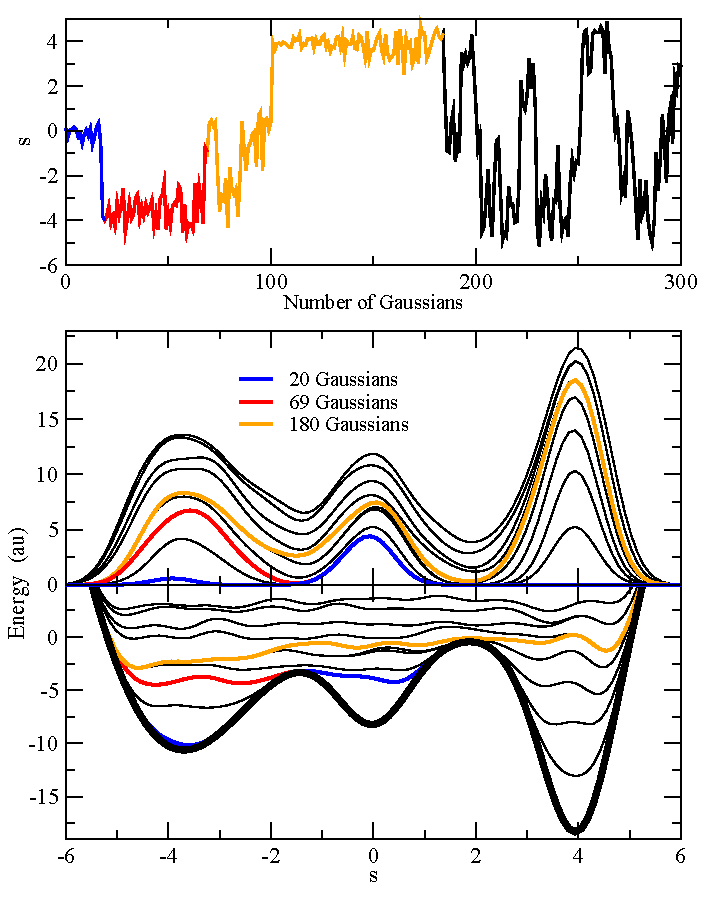
\includegraphics[width=0.55\textwidth]{./img/metadEs}
	\caption{Example of a time evolution of a metadynamics simulation. Top: time evolution of the \acs{CV} of a system evolved on the 3--minima \acs{FES} represented by the black thick line in the lower panel. Middle: time evolution of $w_M$, the history--dependent bias potential. Blue line: $w_M$ when the first minimum is filled and the system escapes to the second minimum; red line: $w_M$ when also the second minimum is filled; yellow line: when the entire profile is filled and the dynamics becomes diffusive on the whole energy landscape. Lower panel: time evolution of the sum of $w_M$ (same color scheme). Taken from \cite{MetadReview}.}
	\label{fig:metadEs}
\end{SCfigure}

Keeping in mind figure~(\ref{fig:metadEs}) a summary of the behavior of metadynamics and the validity of
equation~\eqref{eq:metadfes} can be qualitatively understood in the limit of slow deposition. This means that
$w_M(\vec s, t)$ varies slowly and the probability to observe $\vec s$ is approximately proportional to the
Boltzmann factor $e^{-\beta(G(\vec s) - w_M(\vec s, t))}$. If the function in the exponential has some local
minimum due to $G(\vec s)$, $\vec s$ will preferentially be localized in the neighborhood of this minimum and an
increasing number of Gaussians have to be added until it is completely filled. When the minimum is filled the
system reaches the condition $G(\vec s) \sim w_M(\vec s, t)$, the probability distribution would be approximately
flat and we can say that the system becomes diffusive in the region explored by the simulation. Then, in this
region, the placement of new Gaussians is no more affected by the difference between $G(\vec s)$ and
$w_M(\vec s, t)$ and they are deposited randomly over the flat free energy profile. The \acp{FES} reconstructed
after that point, as visible in figure~(\ref{fig:metadEs}), are affected by some corrugations, due to newly
deposited Gaussians, of the order of $w$. From that point the metadynamics has reached the \textit{convergence}
in the sampled region.

\paragraph{\textbf{convergence}} As just explained before, the convergence of the metadynamics in a specific
region of the \acp{CV} space is reached when the system become diffusive in this region, i.e. when the \acp{CV}
can assume all possible values compatible to the sampled region. This is a crucial point for the metadynamics
method in order to obtain the best possible estimator of the \ac{FES}, in the sampled region. Clearly, in order
to save computational time, if one want only to give the possibility to the system to escape from an energy
minimum is not necessary to reach the convergence otherwise it is an important point. Unfortunately in most
systems it is not trivial to identify precisely when the diffusive regime has been reached. In most cases a
practical method to assess the convergence of metadynamics simulations is based on monitoring the free energy
difference between two reference point: when the difference is approximately flat then the convergence should be
reached.

\paragraph{\textbf{error estimation}} After convergence is reached the error on the \ac{FES} estimator is clearly
dependent on the chosen parameters. The best way to estimate the statistical error introduced by the metadynamics
is to perform several statistically independent metadynamics runs. The arithmetic average of all the
history--dependent potentials taken at the same time, after the convergence is reached, is equal to the best
estimate of the \ac{FES}. The statistical error of the \ac{FES} of a run can be considered as the standard
deviation between the history--dependent potential $w_M(s,t)$ of that run and the averaged \ac{FES}
$G(\vec s) \sim - \overline{w_M(\vec s,t)}$ and average it over the whole \acp{CV} space, as follow
\begin{equation*}
\overline{\epsilon}^2 = \frac{1}{\Omega_s} \int_{\Omega_s}  \overline{(w_M(\vec s,t) - \overline{w_M(\vec s,t)})^2}\ ds
\end{equation*}
where $\Omega_s$ is the whole \acp{CV} space. Laio \etal\, in \cite{MetadError}, by performing extensive
numerical simulations of a Langevin stochastic system, have derived an approximate expression for the error
estimator in function of the system and metadynamics parameters, as follow
\begin{equation*}
	\overline{\epsilon}^2 \propto \frac{LT}{D}\frac{w}{\tau} \delta s
\end{equation*}
where $L$ is the size of the simulation box, $D$ is the system diffusion coefficient and $T$ is the system
temperature. Since $\delta s$ is approximately fixed by the fluctuation of the \acp{CV} in a unbiased \ac{MD} run
and/or by the granularity to be achieved in the \ac{FES} estimator, the error is dominated by the ratio $w/\tau$.
Thus a fine tuning of the Gaussians height and deposition pace is often needed in order to minimize the
statistical error. Despite this, it is commonly accepted to follow a procedure for the \ac{FES} and error
estimators:
\begin{itemize}
	\item Several statistically independent metadynamics simulations are performed;
	\item After the convergence is reached for each run, the estimator of the \ac{FES} is the arithmetic average of the \ac{FES} obtained from equation~\eqref{eq:fes} for each simulations (each free energy profile appropriately normalized);
	\item The statistical error on the averaged \ac{FES} is performed considering its standard deviation.
\end{itemize}
Alternatively one can perform a very long metadynamics run in which, for example, the system is diffusive for
half simulation. Then one can chose as statistically independent history--dependent potentials some of them
computed at different times in the diffusive region and follow the above procedure from the second point. Clearly
one has to be careful about the decorrelation time between the chosen profiles, otherwise they are not
statistically independent due the continuos nature of the metadynamics algorithm.

\paragraph{\textbf{performance optimization}} In general the computational overhead of adding metadynamics to an
\ac{MD} simulation is usually not excessive, even if it depends on the implemented algorithms. However as the
number of deposited Gaussians increases, in each \ac{MD} step a larger and larger number of exponential terms
have to be computed and summed in order to calculate the derivative of the history--dependent potential, i.e. the
forces due to the metadynamics. Thus if the Gaussians are big or frequently deposited or the system takes a lot
of time to reach the convergence, the computational overhead scales as the number of the deposited Gaussians.
This can clearly lead to a loss of performance as the simulation time increase. A simple solution is to implement
a discrete mesh grid on the \acp{CV} space in which the history--dependent potential is spread and stored. When a
new Gaussian is added the potential is updated in the whole grid. While, at each \ac{MD} step, in order to
compute the derivative, the potential in a non--grid point is only estimated from an interpolation of some
neighbor grid points, depending on the interpolation order. By this trick the computational overhead remains
approximately constant as the simulation time increase.

\subsection{Umbrella sampling and metadynamics remarks}
The use of metadynamics is growing up in the computational community. The most relevant reasons are its
simplicity of implementation and the direct way to control the efficiency and performance by changing the
parameters of the Gaussians entering in the history--dependent potential. This gives to the metadynamics the
possibility, with only one framework, to overcome different situations such as passing continuously from a fast
and coarse exploration of the energy landscape to an accurate evaluation of the free energy profile, predict new
stable configurations and structures, new reaction pathways, calculate free energy profiles and free energy
differences.

The main difference of metadynamics respect to umbrella sampling is the process of reconstruction of the free
energy profile. In the latter it follows a predefined scheme designed for covering only the \ac{CV} space along
the chosen path. In contract a well implemented metadynamics reconstruct efficiently the free energy profile:
starting from the current minimum it explore a larger and larger region of the \acp{CV} space in order to
recursively reconstruct the \ac{FES}. However a careful choice of the \acp{CV} is needed, otherwise the
history--dependent potential and the \ac{FES} can evolve in an unphysical manner.

In a recent work by Davide Bochicchio \etal\, \cite{metaUSComparison} both methods for the \ac{FES} estimation
included the error estimation, performance and accuracy are extensively compared with \ac{MD} simulations
involving the transfer of hydrophobic oligomers from the water phase to the hydrophobic core of a lipid membrane.
The authors consider the system both at atomistic and \ac{CG} levels (\martini \ac{FF}). They found that, if the
\acp{CV} are properly chosen and the parameters for the metadynamics are carefully tuned, the reconstructed free
energy profiles are identical between umbrella sampling and metadynamics, but the latter yields the same accuracy
in less simulated time.
